\documentclass[../main.tex]{subfiles}
\graphicspath{{\subfix{../Figures/}}}

\begin{document}

\chapter{Experiments and results}

We now present our experiments to address the problems stated in \autoref{ch:methods}.

First we give details on settings common to all experiments, next we present our metrics of choice
and then we delve into the experiments themselves, presenting the experimental setup, the results and
discussion for each of them in turn.

\section{Datasets}
\label{sec:datasets}

In our experiments we use one custom synthetic dataset generated in a parametrizable way, as well as some real datasets.

We always take out the categorical features and we standardize each feature.

\subsection{\CakeOnSea}

Our analyses are complicated by the impossibility of visualizing counterfactuals for tabular data in general.
Thus, in order to start approaching the problem intuitively, one of our datasets is a synthetic dataset with no more than two features having an influence on the response.
The two features, denoted by $x_0$ and $x_1$, range from 0 to 50, except for the so-called ``dead zone'' which is $[25, 35]^2$, in which there are no points at all.
There are three classes, and the class decision rule is as follows:
\begin{align*}
    (x_0, x_1) \in [35, 45]^2 \implies & y = 2 \\
    x_1 < 25                  \implies & y = 0 \\
    (x_0, x_1) \in \text{dead zone} \lor (x_0, x_1) \notin [0, 50]^2  \implies & y\ \text{unknown} \\
    \text{otherwise} \qquad            & y = 1
\end{align*}
Note that we explicitly refrain from assigning a class to points in the dead zone or outside $[0, 50]^2$.
The decision rule can be visualized in \autoref{fig:cake_on_sea}.

To generate the dataset, we randomly sample points in the $[0, 50]^2$ square and then take out points from the dead zone. By default, the sampling distribution is a uniform $\mathcal{U}([0, 50]^2)$.

Our implementation also allows for producing more features that are linear combinations of the first two, to simulate data with an arbitrary number of columns while keeping the dataset structure intact.
However, in the interest of keeping things simple, we use only the 2-feature version in our analyses.

\begin{figure}[h]
    \centering


\tikzset{every picture/.style={line width=0.75pt}} %set default line width to 0.75pt        

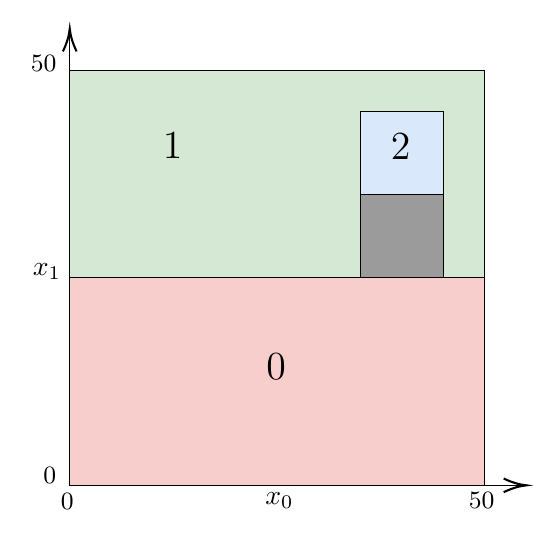
\begin{tikzpicture}[x=0.75pt,y=0.75pt,yscale=-1,xscale=1]
%uncomment if require: \path (0,300); %set diagram left start at 0, and has height of 300

%Shape: Rectangle [id:dp12943827359599314] 
\draw  [fill={rgb, 255:red, 213; green, 232; blue, 212 }  ,fill opacity=1 ] (250,50) -- (450,50) -- (450,150) -- (250,150) -- cycle ;
%Straight Lines [id:da8416607833401318] 
\draw    (250,250) -- (250,32) ;
\draw [shift={(250,30)}, rotate = 90] [color={rgb, 255:red, 0; green, 0; blue, 0 }  ][line width=0.75]    (10.93,-3.29) .. controls (6.95,-1.4) and (3.31,-0.3) .. (0,0) .. controls (3.31,0.3) and (6.95,1.4) .. (10.93,3.29)   ;
%Straight Lines [id:da5577600596159713] 
\draw    (250,250) -- (468,250) ;
\draw [shift={(470,250)}, rotate = 180] [color={rgb, 255:red, 0; green, 0; blue, 0 }  ][line width=0.75]    (10.93,-3.29) .. controls (6.95,-1.4) and (3.31,-0.3) .. (0,0) .. controls (3.31,0.3) and (6.95,1.4) .. (10.93,3.29)   ;
%Straight Lines [id:da17568384394881242] 
\draw    (250,150) -- (450,150) ;
%Shape: Rectangle [id:dp3705541448905584] 
\draw  [fill={rgb, 255:red, 248; green, 206; blue, 204 }  ,fill opacity=1 ] (250,150) -- (450,150) -- (450,250) -- (250,250) -- cycle ;
%Shape: Rectangle [id:dp5334639009219723] 
\draw  [fill={rgb, 255:red, 218; green, 232; blue, 252 }  ,fill opacity=1 ] (390,70) -- (430,70) -- (430,110) -- (390,110) -- cycle ;
%Shape: Rectangle [id:dp05533155300504711] 
\draw  [fill={rgb, 255:red, 155; green, 155; blue, 155 }  ,fill opacity=1 ] (390,110) -- (430,110) -- (430,150) -- (390,150) -- cycle ;

% Text Node
\draw (343.5,185.33) node [anchor=north west][inner sep=0.75pt]  [font=\Large]  {$0$};
% Text Node
\draw (293.6,79) node [anchor=north west][inner sep=0.75pt]  [font=\Large]  {$1$};
% Text Node
\draw (403.5,79.33) node [anchor=north west][inner sep=0.75pt]  [font=\Large]  {$2$};
% Text Node
\draw (343,252) node [anchor=north west][inner sep=0.75pt]    {$x_{0}$};
% Text Node
\draw (231,142) node [anchor=north west][inner sep=0.75pt]    {$x_{1}$};
% Text Node
\draw (244.5,252.67) node [anchor=north west][inner sep=0.75pt]  [font=\small]  {$0$};
% Text Node
\draw (236,240.33) node [anchor=north west][inner sep=0.75pt]  [font=\small]  {$0$};
% Text Node
\draw (230,41.67) node [anchor=north west][inner sep=0.75pt]  [font=\small]  {$50$};
% Text Node
\draw (441,252) node [anchor=north west][inner sep=0.75pt]  [font=\small]  {$50$};


\end{tikzpicture}

\caption{Decision rule for the \CakeOnSea dataset. The so-called ``dead zone'' is shown in dark gray between class 2 and class 0.}
    \label{fig:cake_on_sea}
\end{figure}

\subsection{\ForestCover}

This dataset is taken from the UCI Machine Learning repository\footnote{\url{https://archive.ics.uci.edu/ml/datasets/Covertype}} \cite{duaUCI2019} based on work in \cite{blackardComparative1999}.
It contains data on 581012 trees such as their elevation, their horizontal distance to the nearest surface water features and the type of soil they are in, as well as their species, among seven tree species. There is a total of 13 recorded variables, including the tree species. Of the 12 variables used for prediction, two are categorical, and encoded as one-hot columns.
Because our method does not trivially extend to categorical features yet, we remove the one-hot columns; we thus have $D = 10$.

\subsection{\WineQuality}

The \WineQuality{} dataset originates from \cite{cortezModeling2009} and can be found in the UCI repository\footnote{\url{https://archive.ics.uci.edu/ml/datasets/Wine+Quality}}.
It consists of data on 6498 Portuguese ``Vinho Verde'' wines, such as their pH, their density and their alcohol percentage, as well as a quality rating from 0 to 10.
There are 13 variables including the quality rating column; except for the quality and whether they are red or white, all of them are numerical.
As before, we remove the red/white information.

Because the wine quality is an ordinal variable (categorical but ordered), it is not necessarily appropriate to run a classifier on the dataset directly;
thus, we group quality ratings together into 3 classes.
In fact, there are no wines with a quality rating of 0, 1, 2 or 10, and 43\% of the rows have a rating of 6 out of 10.
Hence, for our classification task we create the following class mapping:
\begin{itemize}
    \item class 0 corresponds to a quality rating of 5 or lower (33\% of the data),
    \item class 1 to a rating of 6 (43\%) and
    \item class 2 to a rating of 7 or higher (18\%).
\end{itemize}

\subsection{\OnlineNewsPopularity}

This dataset \cite{fernandesProactive2015} also from the UCI repository\footnote{\url{https://archive.ics.uci.edu/ml/datasets/Online+News+Popularity}} contains data on 39644 news posts recovered from the Mashable website, such as the number of HTML tags of a certain type, the time of publishing, and also machine-learning-derived features such as the subjectivity and polarity of the language used, and how well the post fits within a given topic as determined by LDA.
As before, we remove the categorical columns, leaving us with 46 columns including the target variable.

The target variable is the number of shares of a given article, which is an integer; in order to make it usable for classification tasks, we create the following class mapping:
\begin{itemize}
    \item Articles with a number of shares below the median (\ie{} in the worst 50\%) are considered to be in class 0,
    \item Articles between the 50\% and the 75\% percentiles are considered class 1,
    \item Articles between the 75\% and 95\% percentiles are considered class 2,
\item Articles above the 95\% percentile (\ie{} in the best 5\%) are considered class 3.
\end{itemize}
Thus, class 0 contains 50\% of the data, class 1 contains 25\%, class 2 contains 20\% and class 3 contains 5\%.

\subsection{Summary of datasets}

All datasets are divided into training, validation, and test sets containing 60\%, 20\%, and 20\% of the data respectively.

In \autoref{tab:datasets} we summarize the relevant information about our datasets and settings when using them for training.

\begin{table}[h!]
    \centering
\begin{tabular}{lrrrrrr}
        \toprule
Name          & $\inputdim$ & $\outputdim$ & $\card{\trainset}$     & $\card{\valset}$     & $\card{\testset}$    & $
\card{\trainset} / \inputdim$  \\
        \midrule
\CakeOnSea            & 2           & 3            & 57607                  & 19202                & 19202        & 28803                    \\
\ForestCover          & 10          & 7            & 348608                 & 116202               & 116202       & 34861                   \\
\WineQuality          & 11          & 3            & 3900                   & 1299                 & 1299          & 355                  \\
\OnlineNewsPopularity & 45          & 4            & 23788                  & 7928                 & 7928          & 529                   \\
        \bottomrule
    \end{tabular}
    \caption{Summary of our dataset settings. $\inputdim$ refers to the number of features, $\outputdim$ to the number of classes, and $\abs{\trainset}$, $\abs{\valset}$, $\abs{\testset}$ to the size of the train, validation, and test set respectively.}
    \label{tab:datasets}
\end{table}

\section{Models}

All models are trained using the Adam algorithm \cite{kingmaAdam2014} with a learning rate of $1 \times 10^{-3}$.
We let the models train for an undetermined number of epochs, performing early stopping based on the validation loss with a patience parameter of 3.

The models are implemented in \texttt{pytorch} and trained on a machine with the following characteristics:
\begin{itemize}
    \item CPU: Intel Core i7-7700K CPU @ 4.20GHz
    \item RAM: 32 GB
    \item GPU: Nvidia G-Force GTX 1080 via CUDA 11.7
\end{itemize}

\subsection{Classifier}
\label{exp/classifiers}

The classifier architecture in our analyses is an MLP consisting of two 50-node linear layers each followed by a $\relu$, then one last linear layer outputting $\outputdim$ logits.

In \autoref{fig:confusion_matrices} we show the test predictions of our classifier architecture, trained with batch sizes:
\begin{itemize}
    \item \CakeOnSea: 12000
    \item \ForestCover: 25000
    \item \WineQuality: 500
    \item \OnlineNewsPopularity: 3000
\end{itemize}
The batch sizes are chosen so that one epoch takes less than 10 steps, except for \ForestCover{} where the size of the train set would have resulted in very large batches.
In each experiment we ended using different batch sizes so we re-state them when appropriate.

\begin{figure}
    \centering
    \begin{subfigure}[b]{0.4\textwidth}
        \centering
\includegraphics[width=\textwidth]{./05_confusion_matrices/cake_on_sea/confusion_matrix_svg-tex.pdf}
        \caption{Accuracy on \CakeOnSea.}
\label{fig:cos_confusion_matrix}
    \end{subfigure}
    \begin{subfigure}[b]{0.4\textwidth}
        \centering
\includegraphics[width=\textwidth]{./05_confusion_matrices/forest_cover/confusion_matrix_svg-tex.pdf}
        \caption{Accuracy on \ForestCover.}
    \end{subfigure}

    \begin{subfigure}[b]{0.4\textwidth}
        \centering
\includegraphics[width=\textwidth]{./05_confusion_matrices/wine_quality/confusion_matrix_svg-tex.pdf}
        \caption{Accuracy on \WineQuality.}
    \end{subfigure}
    \begin{subfigure}[b]{0.4\textwidth}
        \centering
\includegraphics[width=\textwidth]{./05_confusion_matrices/online_news_popularity/confusion_matrix_svg-tex.pdf}
        \caption{Accuracy on \OnlineNewsPopularity.}
    \end{subfigure}

    \caption{Accuracy of our MLP classifier on each dataset.}
    \label{fig:confusion_matrices}
\end{figure}

It seems the classifier achieves low accuracy on \WineQuality{} and \OnlineNewsPopularity{} in particular.
These datasets are originally designed for regression, so they are perhaps not well suited for classification tasks; however, their size is also likely a factor: they have on the order of $10^2$ training examples per dimension where the others have on the order of $10^4$.

All datasets also have significant class imbalance: in \ForestCover{} the test set contains 56382 points with true class 1 while only 554 points in class 3.

\subsection{Autoencoder}

We build a normalizing flow model according to the NICE architecture described in \autoref{bg/nf} \cite{dinhNICE2015}.
The model is trained according to a Gaussian prior distribution, and its layers are 4 additive coupling layers where we divide the input into the odd columns and the even columns, and the nonlinearity in each coupling layer is an MLP with 2 layers of 20 nodes each.

\section{Metrics}

In this section we describe the various metrics that will be used in some or all of our experiments.

\subsection{Validity}

Validity is the one requirement where the metric of interest is unambiguous: either a path is valid or it is not.
Hence, for testing a path generation method on some test set, we measure the validity rate, which is the proportion of valid paths.

\subsection{Computational performance}

Ensuring that CFX generation is fast is an important concern for stakeholders, especially if one needs to generate paths for many points of interest.
Hence, we measure the time taken \emph{for one step of one path}.
This is because depending on the number of steps chosen by the user, a path can take longer to generate, and methods such as \ls{} can take advantage of optimizations to compute many paths at once.

\subsection{Realism}

Following the reasoning presented in \cite{vanlooverenInterpretable2021}, we measure realism using a generative model.
However, while \citeauthor{vanlooverenInterpretable2021} use a VAE and thus estimate realism using the reconstruction error, we can compute the likelihood directly.
Indeed, normalizing flows are typically trained to minimize the $\nll = - \log P(x)$, so we can compute it easily.
$P(x)$ is in non-negative so the $\nll$ is in $\R_+$ and the closer it is to 0, the more realistic the point is deemed to be.

For some time we also used the local outlier factor \cite{breunigLOF2000}, for which an implementation is provided by the \sklearn{} Python package, but it did not scale to all of our datasets.

\subsection{Extending metrics to a path}
\label{exp/masking}

All the CFX paths are 100 points long (including the starting point, so the number of steps is 99) and the step size $\lambda_\text{LS}$ is 0.1. We found this to be satisfactory so that the path is long enough to reach the target class, yet with step size short enough that the path does not go too far too quickly.

Many metrics take a point $x' \in \inputspace$ as input and return a score, but in our case we wish to score a whole path $(x_t)_{t=1}^T$.
Hence, given a metric, we aggregate over the path (that is, from its starting point to the first step at which $\target$ is reached).

For this, we first produce paths in the form of a 3-dimensional tensor in $\R^{\nbsteps \times \batchsize \times \inputdim}$,
where $\nbsteps$ is the number of steps in the path and $\batchsize$ the batch size.
We compute the model predictions resulting in a 2-dimensional tensor in $\setclasses^{\nbsteps \times \batchsize}$.
Based on this and the target classes we generated in $\setclasses^\batchsize$, we construct a mask $\pathmask \in \{0, 1\}^{\nbsteps \times \batchsize}$ that highlights the valid paths:
if path $j$ is not valid, then
$\forall i \in \{1, \ldots, \nbsteps\}$ ${\pathmask_{ij} = 0}$, and if path $j$ is valid then $\pathmask_{ij} = 1$ up to and \emph{not including} the first index where $\target$ is reached, and 0 after that.

Then we can take the element-wise product of, \eg{} the $\nll$ computed for all points of all paths, to mask the unwanted points.

Note that if no paths are valid, the resulting product will be equal to zero, which can be misleading: $\nll = 0$ is a perfect score.
For this reason we take care to always report the validity rate alongside any metric computed this way.

Let us now describe our experiments in detail.

\section{Experiment 1: Validity losses}

In this experiment, we seek to determine the validity loss that maximizes validity rate among a number of choices.
For this we measure the validity rate over CFs generated from the test set across several CF methods and losses.

\paragraph{Description}
\label{validity_losses/description}

For a given dataset, we train one classifier.
Then for this dataset, we train several autoencoders all with the same architecture and with different seeds to average out random effects due to model initialization and dataset train-test split.
The seeds are generated uniformly based on one primary seed.

For a given dataset, we measure the validity rate across the whole test set.
That is, for every test point, we run the classifier to get the $\source$ class ($\source = \arg\max_{c \in \setclasses} f(x)$), and we sample the target class uniformly from $\setclasses \backslash \{\source\}$.
Then we generate a path using the given loss $\lossval$, and count it as valid or not.
It is important to sample the $\target$ uniformly to get a full understanding because, even when the label distribution is not uniform, in general there is no reason to prefer explanations for a given target rather than another.

We average the rates over the different seeds, and report the standard error.

\paragraph{Baselines}

The methods we use to produce the paths are variations on \ls{} and \revise{}.
To compare methods on a par, we run both methods twice: once with regularization on the $L_1$ distance, with $\lambda_\text{distance} = 0.3$ and once without regularization (with $\lambda_\text{distance}$ set to 0).
In the future using some automatic tuning procedure would be best: in our case $\lambda_\text{distance} = 1$ led to immobile paths whereas $\lambda_\text{distance} = 0.3$ could be too close to performing no regularization at all.

In fact, our implementation of both \ls{} and \revise{} is a joint abstraction that takes a parameter for the frequency of the gradient computation: for \revise{} this is set to 1 (\ie{} recompute the gradient after every step) while for \revise{} it is null (\ie{} never recompute it).
This way the number of steps and step size can be set to the same values with confidence.
However, this means that we do not run \revise{} using a more sophisticated optimization algorithm like \method{Adam} or \method{RMSprop}.

The losses compared in this experiment are as follows:
\begin{itemize}
    \item The probability-based losses: $\PrbTarget, \PrbSource{}$
    \item The log-probability-based losses: $\LogPrbTarget, \LogPrbSource{}, \LogPrbOthers{}$
    \item The logit-based losses: $\LogitTarget, \LogitSource{}, \LogitOthers{}$
\end{itemize}
where we test all losses that can be parametrized with the default parameter of $\lambda = 1$ and also with $\lambda = 0.1$, for a total of 13 losses ($\PrbTarget$ is not parametrized, and recall that $\PrbOthers{}$ is equivalent to $\PrbTarget$.).
Here again, a larger scale parameter search should have been done, but instead we first select the best-performing loss and then show the progression for $\lambda \in [0, 1]$.

\paragraph{Datasets}

We run our experiment on the datasets described in \autoref{sec:datasets}, namely \CakeOnSea, \ForestCover, \WineQuality{} and \OnlineNewsPopularity.

The batch sizes are chosen so that one epoch takes less than 10 steps, except for \ForestCover{} where the size of the train set would have resulted in very large batches.
The final numbers are:
\begin{itemize}
    \item \CakeOnSea: 12000
    \item \ForestCover: 25000
    \item \WineQuality: 500
    \item \OnlineNewsPopularity: 3000
\end{itemize}

\paragraph{Metrics}

The one metric in this experiment is the validity rate, \ie{} the proportion of paths that reach their target class across the whole test set.

\paragraph{Results}

The results for each dataset and loss are given in \autoref{tbl:validity_losses}.
We highlight in gray the five losses that yield the best average validity rate across all path methods; the results are not uniform across datasets so we resort to this rough estimate to decide between the losses.

\begin{table}[h!]
\centering
\subfile{../Figures/05_validity_losses.tex}
\caption{Validity rate means with their standard error. Highlighted for each dataset are the five losses with the best average results.}
\label{tbl:validity_losses}
\end{table}

The validity rate achieved by \revise{} is generally much more acceptable than that of \ls{}, across all losses.
This is expected given that \revise{} can correct its trajectory as the path is generated, while \ls{} cannot.

$\LogitSource{}$ is always among the best validity losses.
However, it is not always clear which value of $\lambda$ should be used.
Hence, we show the validity rate for $\lambda \in \{ 0.01, 0.05, 0.1, 0.2, 0.5, 1\}$ in \autoref{fig:lambda_progression}.

\begin{figure}[htbp]
    \centering
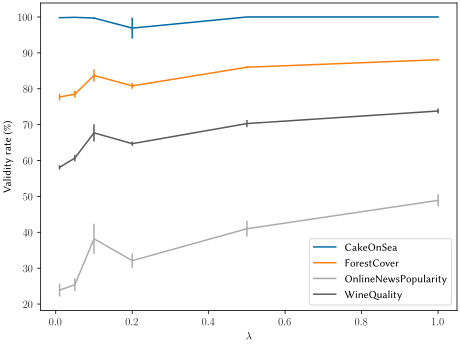
\includegraphics[width=0.7\textwidth]{./05_logit_source_lambda_progression}

    \caption{Validity rate for $\LogitSource{\lambda}$ for different values of $\lambda$.}
    \label{fig:lambda_progression}
\end{figure}

From this plot it is clear that in general letting $\lambda = 1$ leads to higher validity rate;
however the validity is unusually high for $\lambda = 0.1$ compared to the others.

To make better sense of our findings given our considerations on gradients in \autoref{sec:validity_losses},
we also plot our various losses and their gradients on \CakeOnSea.
Here, we select plots for some losses and where the target class is always class 2.
For reference, the full plots are shown in \autoref{ch:plots}.


\begin{figure}[htbp]
    \centering
\includegraphics[width=\textwidth]{./05_cf_losses/cf_losses_detail}
    \caption{Loss profile for various losses on \CakeOnSea, with ${\target = 2}$.}
    \label{fig:cf_losses_detail}

    \vspace*{\floatsep}% https://tex.stackexchange.com/q/26521/5764

\includegraphics[width=\textwidth]{./05_cf_losses/cf_gradients_detail}
    \caption{Opposite of the loss gradient for various losses on \CakeOnSea, with $\target = 2$.}
    \label{fig:cf_gradients_detail}
\end{figure}

\paragraph{Interpretation}

From the plot values in the probability-based losses in \autoref{fig:cf_losses_detail}, we can tell that for \CakeOnSea{} the prediction probabilities are all close to 1, except perhaps near the decision boundaries.
Hence, we can verify our intuitive thinking from \autoref{sec:validity_losses}: for the probability-based losses, the loss is very flat, \ie{} the gradient is close to zero.
For $\LogPrbOthers{}$ it seems the logits from the other classes counteract the target logit, so that paradoxically the paths get pushed away from class 2 in places.
For the logit-based losses however, the behavior is fairly uniform across the whole data distribution, and so the gradients clearly point the path towards class 2.

This leads us to choose $\LogitSource{\lambda=1}$ as validity loss in the rest of our analyses.

\section{Experiment 2: Path regularized training}
\label{exp/path_reg}

Having determined an appropriate validity loss to use for generating valid paths, we turn now to our objective of interpretability.
In this experiment we seek to determine if \ls{} equipped with a path regularized autoencoder can perform on the same level as \revise{}, increasing interpretability without compromising validity.

Our proxy for interpretability of a path is \emph{the number of class boundary crossings}:
the path should ideally transition from $\source$ to $\target$ without going through other classes.
We thus add our $\BoundaryCrossLoss$ to the $\nll$ when computing the loss of the autoencoder.
Our final loss for training the autoencoder is
\begin{align*}
    \loss_\text{NF}(\phi) = \nll(\phi) + \BoundaryCrossLoss(\apath)
\end{align*}
where $\apath$ is a path generated with some CF method.


\paragraph{Description}

First, we generate some seeds.
For a given dataset, we train one classifier, as in \autoref{validity_losses/description}.
Then, for each path method and seed, we train two autoencoders: with and without path regularization.

Then, each autoencoder is used to produce explanation paths on the whole test set, like in \autoref{validity_losses/description}, and metrics are computed with the paths as input.
Finally, for each explanation method, we aggregate the metrics obtained for each seed and report the standard error.


\paragraph{Baselines}
\label{exp/path_reg/baselines}

Since the distance parameter seems inconsequential from our previous results,
in this experiment we use \ls{} and \revise{} in their basic form, \ie{} with no distance regularization for \ls{} and with $\lambda_\text{distance} = 0.3$ for \revise.

\paragraph{Datasets}

For memory performance reasons (the loss involves paths in the form of three-dimensional tensors) we reduce the batch size for each dataset compared to the previous experiment.
We compute the batch size so that one training epoch (one pass through $\trainset$) takes 20 steps, except for \ForestCover{} where the batches are still too big.
The final numbers are:
\begin{itemize}
    \item \CakeOnSea: 2881
    \item \ForestCover: 5000
    \item \WineQuality: 195
    \item \OnlineNewsPopularity: 1190
\end{itemize}

\paragraph{Metrics}

We measure the validity rate, as before, as well as the number of boundary crossings \emph{before reaching $\target$} (so if the path goes directly from $\source$ to $\target$ the value is 0) which is the proxy for interpretability we chose.
For this we use the masking procedure described in \autoref{exp/masking}.

For measuring realism, we use a specially-trained autoencoder with the same architecture as the others, trained using only the $\nll$ as a loss.
The realism score for $\CF{x}$ is given by its $\nll$ as computed by our special autoencoder;
the metric is extended to the paths using path masking again.

We also measure the computational complexity (the duration for one computing one step of one path).

\paragraph{Results}

The results for each dataset and method are given in \autoref{tbl:path_reg}.

\begin{table}[h!]
    \centering
    \subfile{../Figures/05_path_reg.tex}
    \caption{Path metrics with their standard error. ($\uparrow$) indicates higher is better, ($\downarrow$) indicates lower is better.}
    \label{tbl:path_reg}
\end{table}

It seems the regularization did not achieve its objective, as the mean number of boundary crossings stays approximately the same regardless of whether or not regularization was performed.
The only case where an effect is observed is for \revise{} on \CakeOnSea{}.
In no instance do we see a decrease in validity rate when applying path regularization.
Similarly, path regularization by and large has no effect on realism, except for \ls{} on \CakeOnSea{} and \ForestCover{} where the $\nll$ is decreased when applying regularization.
The time per step does not depend on the autoencoder training, only on the architecture.
Yet, we can observe the difference in time performance between \ls{} and \revise{}: \ls{} is up to 70 times faster than \revise{} on \OnlineNewsPopularity{}.

\paragraph{Interpretation}

The regularization was not strong enough to alter the training of the autoencoder.
Recall our loss function is given by
\begin{align*}
    \BoundaryCrossLoss(\apath) =
    - \frac{1}{\nbsteps} \sum_{t=1}^{\nbsteps}
    \max \{ p^{(t)}_\source, p^{(t)}_\target \}
\end{align*}
which is in $[-1, 0]$.
By contrast, the $\nll$ is computed according to a Gaussian prior distribution which can typically be as large as $\latentdim$ (see \autoref{methods:0_sols}), which is larger than 10 for all datasets except for \CakeOnSea{} where $\latentdim=2$.
Therefore, one easy improvement is to multiply the $\BoundaryCrossLoss$ by $\latentdim$.

\section{Experiment 3: Robustness of explanations with path regularization}

Given that we were able to achieve more interpretable paths using path regularization, we ask whether it is possible to meet any interpretability criterion, even a nonsensical one.
For example, can we use path regularization so that all paths pass through one designated point, regardless of $x$ and $\target$, while staying valid?
To do so, we select a point $\xgoal \in \inputspace$ that we can reasonably expect to be unrealistic, but is not completely out of reach compared to points in the train set.
Then, we devise a path loss that encodes the distance from a path to $\xgoal$, and let our path regularization training enforce this constraint.
The loss is computed as:
\begin{align*}
    \pathloss(\xgoal, (z_t)_{t=1}^T) = \min_{t \in \{1, \ldots, T\}} \{ \norm{\dec(z_t) - \xgoal}_2 \}
\end{align*}

\paragraph{Description}

We perform path regularized training using an adversarial path loss.
The loss encodes how close a path passes by a given point $\xgoal$, which is potentially unrealistic.
In our experiment, we pick a $\xgoal$ that is easy to compute, likely unrealistic yet not completely out of bounds for the dataset:
\begin{equation}
    \xgoal = (\max\{ x_i : x \in \trainset \})_{i=1}^D
\end{equation}
\ie{} $\xgoal_i$ is the largest value encountered in the train set for feature $i$.

Apart from this the setup is the same as that described in \autoref{exp/path_reg}, where we compare paths with the distance path regularization and without.

\paragraph{Baselines}

We use the same baselines as in the previous experiment (\autoref{exp/path_reg/baselines}).

\paragraph{Datasets}

We use our datasets with the following batch sizes:
\begin{itemize}
    \item \CakeOnSea: 2881
    \item \ForestCover: 3000
    \item \WineQuality: 195
    \item \OnlineNewsPopularity: 1190
\end{itemize}
We reduced the batch size for \ForestCover{} again for memory performance reasons.

\paragraph{Metrics}

As before, we measure the validity rate, the time performance as well as the $\nll$ (with masking).

In addition, we measure the mean distance from a path to $\xgoal$ \emph{before the target is reached}
using the masking procedure.

\paragraph{Results}

The results for each dataset and method are given in \autoref{tbl:robustness}.

\begin{table}[h!]
    \centering
    \subfile{../Figures/05_robustness.tex}
    \caption{Path metrics with their standard error. ($\uparrow$) indicates higher is better, ($\downarrow$) indicates lower is better.}
    \label{tbl:robustness}
\end{table}

We see that for \CakeOnSea{} and \WineQuality the regularization had little effect.

However, it did induce changes in behavior for the two remaining datasets:
\begin{itemize}
    \item for \ForestCover{} the mean distance decreased and the $\nll$ heavily increased;
    \item for \OnlineNewsPopularity{} the mean distance did not change but the $\nll$ heavily increased.
\end{itemize}

The time measurements are much more reasonable than in the previous experiment, although the trends are the same.

\paragraph{Interpretation}

By and large the regularization did not apply uniformly for all datasets; the distance-based loss
is not bounded to a small interval like the $\BoundaryCrossLoss$, which could have had the opposite
effect of causing the $\nll$ not to be prioritized during training.
More precisely, decreasing the distance should have the effect of increasing the $\nll$;
but if the $\nll$ increases too much then
the total loss will increase, at which point the early stopping mechanism will fire.

Relatedly, the $L_2$ distance naturally grows as $\inputdim$ increases, as a consequence of the curse
of dimensionality; while the $\nll$ is also affected as discussed in the previous experiment, this
could make the training even more unstable.
 
This concludes our experiments in this project.

\end{document}